\chapter{Vorgehen}
\label{chap:vorgehen}
% Dieses Kapitel beschreibt das methodische Vorgehen, welches in der Arbeit angewendet wurde. Erwähnen Sie hier die verschiedenen Phasen der Arbeit und ihre Ergebnisse. Arbeiten mit hohem Softwareentwicklungs-Anteil lehnen sich am besten an eine etablierte Vorgehensweise an wie zum Beispiel Scrum, XP oder Agiler UP. Detailierte Projektpläne, Deliverables und anderes, falls vorhanden, gehören aber in den Anhang.

\section{Arbeitsorganisation}
\label{sec:vorgehen_orga}
Im Vordergrund dieser Diplomarbeit stehen der Prozess der Entstehung eines Expertensystemes sowie die Analyse der dazu benötigten Grundlagen. Der Fokus liegt dabei absichtlich nicht in der Softwareentwicklung. Traditionelle Methoden der Projektorganisation wie HERMES oder Scrum wurden daher nicht gewählt.\\
Der Organisation wurden die im Voraus definierten Meilensteine (Teilziele) zu Grunde gelegt. Jeder dieser Meilensteine wurde zeitlich determiniert. Zugleich wurden die Tätigkeiten für jeden Meilenstein durch eine individuelle Liste verteilt. Der benötigte Zeitaufwand sowie die Tätigkeiten wurden durch ein gemeinsames Journal erfasst, siehe~\ref{chap:arbeitsjournal}.

Ein wichtiger Teil der Arbeit ist das Dokument, welches gewonnene Erkenntnisse festhält. In diesem Dokument wurden Erfolge und Misserfolge beschrieben und analysiert. Es bildet schliesslich die Grundlage für das vorliegende Abschlussdokument (bei Anfrage jederzeit verfügbar).

\subsection{Regelmässige Treffen}
\label{sec:vorgehen_orga_treffen}
Regelmässige Besprechungen mit dem Betreuer der Arbeit halfen die gesteckten Ziele zu erreichen und Fehlentwicklungen zu vermeiden. Der Betreuer unterstützte die Autoren dabei mit Vorschlägen. Die Treffen fanden mindestens alle zwei Wochen statt und sie wurden in Form eines Protokolles festgehalten (bei Anfrage jederzeit verfügbar).

\section{Projektphasen}
\label{sec:projektphasen}

\subsection{Meilensteine}
\label{subsec:vorgehen_projektphasen_meilensteine}
Um bei der Arbeit ein möglichst strukturiertes Vorgehen einzuhalten, wurden folgende Projektphasen gewählt:
\begin{itemize}
    \item Projektstart
    \item Erarbeitung und Festhalten der Anforderungen
    \item Erarbeitung der formalen und technischen Grundlagen
    \item Modellierung der Ontologie
    \item Erstellung der Dokumentation zur Wissensmodellierung (Tutorial)
    \item Erstellung des Prototypen der Benutzerschnittstelle
    \item Erstellung der abschliessenden Dokumentation
\end{itemize}

Die gewonnen theoretischen Grundlagen wurden in das Tutorial eingebaut. Sie konnten direkt zur praktischen Umsetzung des Modelles verwendet werden. Bei der Modellierung gewonnene Erkenntnisse ihrerseits konnten direkt in das Dokument übernommen werden. Die drei Phasen liefen dabei parallel ab.

\subsection{Zeitplan/Projektphasen}
\label{subsec:vorgehen_projektphasen_zeitplan}

\begin{figure}[H]
    \begin{ganttchart}[
        vgrid,
        x unit=0.7cm,
        bar/.append style={fill=bfhgrey!50},
    ]{1}{16}
        \gantttitle{2014}{14}
        \gantttitle{2015}{2} \\
        \gantttitlelist{1,...,16}{1} \\ % chktex 11
        \ganttbar{Projektstart}{1}{2} \\
        \ganttbar{Anforderungen}{1}{3} \\
        \ganttbar{Erarbeitung Grundlagen}{1}{10} \\
        \ganttbar{Tutorialdokument}{4}{5} \ganttbar{}{8}{14} \\
        \ganttbar{Modellierung Ontologie}{5}{8} \ganttbar{}{10}{14}\\
        \ganttbar{Umsetzung Prototyp}{9}{14} \\
        \ganttbar{Dokumentation}{1}{2} \ganttbar{}{9}{16} \\
        \ganttbar{Präsentation/Verteidigung vorbereiten}{13}{16}

        % \ganttlink{elem1}{elem2}
        % \ganttlink{elem1}{elem2}
        % \ganttlink{elem2}{elem3}
        % \ganttlink{elem3}{elem4}
        % \ganttlink{elem4}{elem8}
    \end{ganttchart}
    \caption{Zeitplan; Der Titel stellt Jahreszahlen, der Untertitel Semesterwochen dar}
\end{figure}

\subsection{Projektstart}
\label{subsec:projektstart}
In der ersten Phase wurden die Meilensteine der Arbeit identifiziert und skizziert. Um Details der Aufgabe zu verstehen, wurde das notwendige Vorwissen über semantische Datenbanken erarbeitet. Weiter wurde das Grundgerüst dieser Dokumentation erstellt.

\subsection{Anforderungen}
\label{subsec:anforderungen}
In dieser Phase wurde Ziel dieser Bachelor-Thesis festgelegt. Vom Ziel ausgehend wurden die dazu erforderlichen Projektphasen festgelegt. Siehe Dokument in Anhang~\ref{chap:anf}.

\subsection{Formale und technische Grundlagen}
\label{sub:formale_und_technische_grundlagen}
Im Vorprojekt zu dieser Bachelor-Thesis (BTI7302, Projekt 2; bei Anfrage jederzeit verfügbar) wurden die Grundlagen für die Erstellung und Modellierung von Ontologien teilweise erarbeitet. Erforderliche Technologien wurden während dieser Bachelor-Thesis vollständig erarbeitet.

\subsubsection{Formale Grundlagen}
Als formale Grundlagen dienen:
\begin{itemize}
    \item Aufbau und Modellierung von Ontologien~\citep{IspekOntoBedeutung} sowie~\citep{ISpekOntoGeschichte}
    \item RDF-Syntax~\citep{w3rdf} und~\citep{w3rdf_syntax}
    \item Ontologie-Sprache OWL~\citep{w3owl}
    \item Regel-Sprache SWRL~\citep{swrl}
    \item SPARQL-Abfragesprache~\citep{w3sparql_querylang},~\citep{w3sparql_overview}
\end{itemize}

Das Konzept der technischen Umsetzung war durch die oben erwähnte Vorarbeit bereits gegeben.

Es besteht aus zwei Komponenten:
\begin{itemize}
    \item einem Backend\\
        in Form einer semantischen Datenbank, zur Verarbeitung von (Such-) Anfragen
    \item einem Frontend\\
        zur einfachen Handhabung von Abfragen mit entsprechenden Ergebnissen für Anwender
\end{itemize}

\subsubsection{Technische Grundlagen}
\label{ssubsec:vorgehen:grundlagen:technisch}
Ursprünglich wurde für das Backend Apache Stanbol~\footnote{\url{http://stanbol.apache.org}} gewählt. Während der Arbeit erwies sich, dass Apache Stanbol kein geeignetes Produkt für die geplante Umsetzung des Expertensystemes ist.

Hingegen erlaubt die Verwendung der Graphdatenbank Stardog~\footnote{\url{http://www.stardog.com}}:
\begin{itemize}
    \item Ontologien in diversen Formaten zu importieren und exportieren
    \item Abfragen mittels der SPARQL-Abfragesprache zu stellen
    \item Ziehung von Schlüssen bei Abfragen
\end{itemize}
Die Details dazu sind in~\autoref{chap:komponenten} genauer beschrieben.

Bei der Erarbeitung der Grundlagen einigten sich die Autoren, die Modellierung der Ontologie mittels OWL, der meist verwendeten Standard-Sprache vorzunehmen. Eine Ontologie-Datei im OWL-Format wächst gegeben durch ihre Syntax mit zunehmendem Umfang der Ontologie sehr schnell an. Ausserdem ist deren Syntax XML-basiert und damit nicht sehr leserlich.\\
Angesichts dieser beiden Nachteile waren sich die Autoren einig, dass eine Modellierung der Ontologie in der Ontologie-Sprache OWL nur über ein Hilfsmittel vorgenommen werden sollte.

Die Anwendung Protégé der Universität Stanford erwies sich bei der Recherche am geeignetsten. Protégé erlaubt die Modellierung einer Ontologie in Form von Baumstrukturen und den Export der Ontologie in diverse (Datei-) Formate. Weiter bietet Protégé die Möglichkeit, Informationen einer Ontologie mittels der SPARQL-Abfragesprache abzufragen. Durch einen konfigurierbaren Reasoner erlaubt Protégé das Ziehen von Schlüssen. Eine detaillierte Beschreibung findet sich unter~\autoref{sec:komponenten_protege}.

Protégé bietet zum Ziehen von Schlüssen nebst anderen den Pellet-Reasoner an. Die gewählte Graphdatenbank Stardog nutzt ausschliesslich Pellet. Daher wurde Pellet als Anwendung zum Ziehen von Schlüssen gewählt. Eine detaillierte Beschreibung von Pellet findet sich unter~\autoref{subsec:komponenten_reasoner}.

Die Modellierung einer Ontologie ist ein schrittweiser Prozess. Die gewählten Werkzeuge (Protégé und Stardog) gestatten dies, bieten allerdings nur bedingt eine grafische Übersicht (Details siehe~\ref{subsec:komponenten_protege_view}). Um bei der Modellierung nicht von Beginn an an fixe Strukturen gebunden zu sein, wurde früh im Prozess yEd als geeignetes Werkzeug zur grafischen Modellierung gewählt. Bei yEd handelt sich dabei um ein frei verfügbares Werkzeug zur Erstellung und Bearbeitung von Diagrammen. Innerhalb dieses Werkzeuges entwickelten die Autoren eine Konvention für die grafische Darstellung, um eine konstante Modellierung zu erhalten.
\begin{figure}[H]
    \centering \rotatebox{0}{\scalebox{0.3}[0.3]{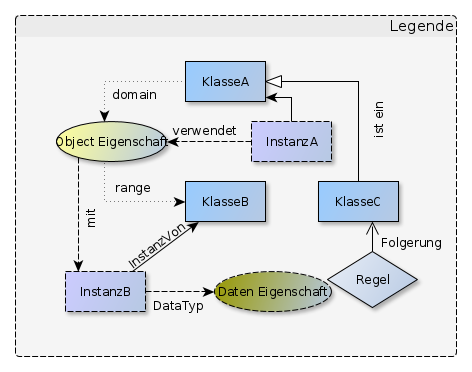
\includegraphics{bilder/yed_legende.png}}}
    \caption{Konvention zur grafischen Darstellung der Ontologie.\label{fig:vorgehen:grundlagen:technisch:yed}\protect\footnotemark}
\end{figure}
\footnotetext{Eigene Darstellung mittels yEd.}

Es bedeuten:
\begin{table}[H]
    \begin{tabular}{m{5em}m{5em}m{5em}m{5em}m{5em}m{5em}}
        \rotatebox{0}{\scalebox{0.3}[0.3]{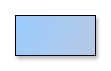
\includegraphics{bilder/yed_konvention_klasse.png}}} & Klasse & 
        \rotatebox{0}{\scalebox{0.3}[0.3]{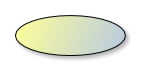
\includegraphics{bilder/yed_konvention_objectprop.png}}} & Objekt-Eigenschaft & \rotatebox{0}{\scalebox{0.3}[0.3]{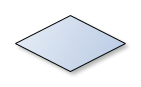
\includegraphics{bilder/yed_konvention_regel.png}}} & Regel \\
        \rotatebox{0}{\scalebox{0.3}[0.3]{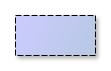
\includegraphics{bilder/yed_konvention_instanz.png}}} & Individuum &
        \rotatebox{0}{\scalebox{0.3}[0.3]{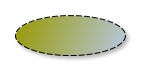
\includegraphics{bilder/yed_konvention_dataprop.png}}} & Daten-Eigenschaft & & \\
    \end{tabular}
\end{table}

Um auch ausserhalb der grafischen Darstellung eine konstante Modellierung zu erhalten, entwickelten die Autoren die folgende Namenskonvention:

\begin{table}[H]%
    \centering
    \begin{tabular}{l l l}
        \toprule{}
        \textbf{Name}       & \textbf{Darstellung/Konvention}       & \textbf{Beispiel}\\
        \midrule{}\\
        Klassen             & Beginnend mit einem Grossbuchstaben   & \textit{Ausflug}\\
        Individuen          & Beginnend mit einem Grossbuchstaben   & \textit{Seilpark}\\
        Objekteigenschaften & Beginnend mit einem Kleinbuchstaben   & \textit{hatStandort}\\
        Dateneigenschaften  & Beginnend mit einem Kleinbuchstaben   & \textit{dauer}\\
        Annotationen        & Beginnend mit einem Kleinbuchstaben   & \textit{url}\\
        \bottomrule{}
    \end{tabular}
    \caption{Namenskonvention der Modellierung}
\label{tab:vorgehen:grndlagen:technisch:konvention}
\end{table}%


\subsection{Modellierung der Ontologie}
\label{sub:modellierung_der_ontologie}

\subsubsection{Vorarbeit für die Modellierung der Ontologie}
\label{sub:modellierung_der_ontologie_vorarbeit}
Ursprünglich wurde versucht ein Modell der (Logik-) Programmiersprache Prolog zu erstellen. Da die Autoren über ein Basiswissen der objektorientierten Programmiersprachen verfügen, wurde UML als Mittel zur Modellierung verwendet. Es zeigte sich rasch, dass es nicht genügt nur Klassen zu definieren; denn eine Ontologie bildet direkte Beziehungen nur zwischen Individuen ab. Die Ontologie muss daher immer über Individuen (Instanzen der Klassen) verfügen.

\begin{figure}[H]
\centering \rotatebox{0}{\scalebox{0.3}[0.3]{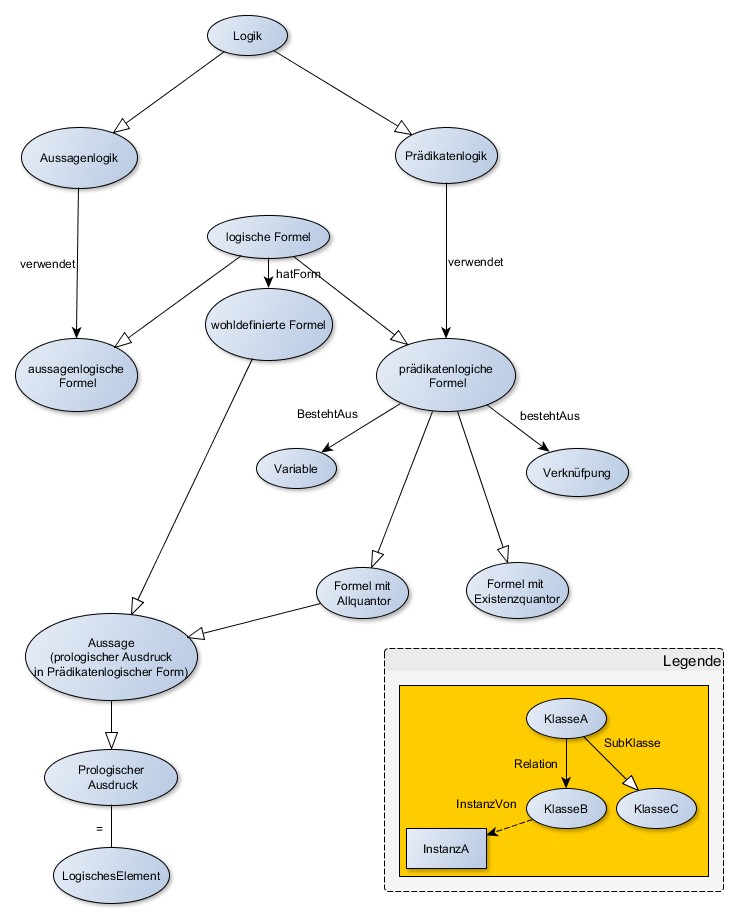
\includegraphics{bilder/formel_baum.png}}}
\caption{Vereinfachte Darstellung von Logik, rein mittels Klassen.\label{fig:prolog_logik_baum}\protect\footnotemark}
\end{figure}
\footnotetext{Eigene Darstellung mittels yEd.}

\newpage

Angesichts dieser Erkenntnis wurde die Modellierung mit Individuen erweitert. Dies ermöglicht die Verwendung von Relationen zwischen Individuen, was richtungsweisend war.

\begin{figure}[H]
\centering \rotatebox{0}{\scalebox{0.3}[0.3]{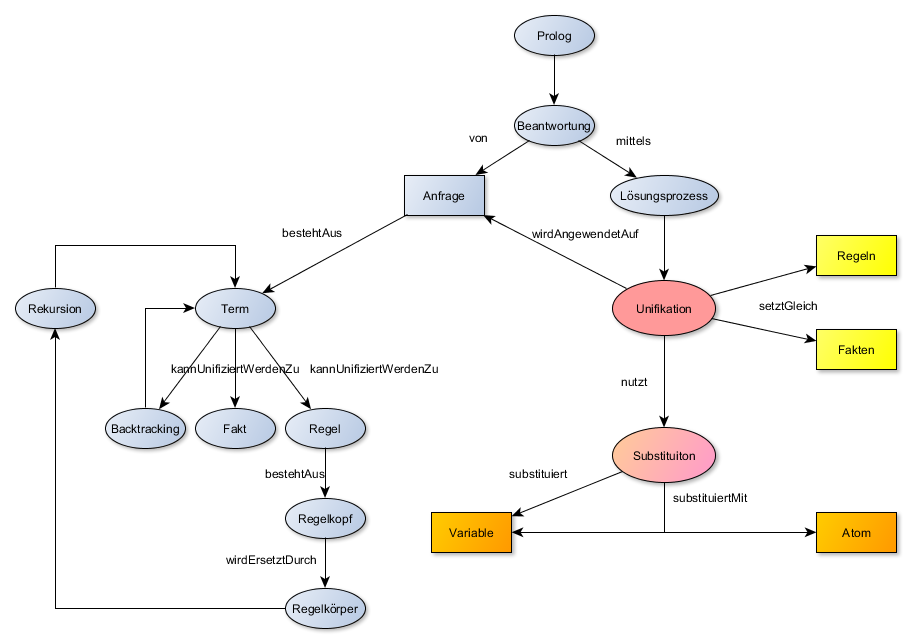
\includegraphics{bilder/loesungsprozess_baum.png}}}
\caption{Vereinfachte Darstellung eines Teils des Lösungsprozesses von Prolog, mittels Klassen, Individuen und Relationen.\label{fig:prolog_loesungsprozess}\protect\footnotemark}
\end{figure}
\footnotetext{Eigene Darstellung mittels yEd.}

Aufgrund der erstellten, bisherige Ontologie konnten konkrete Fragen nicht beantwortet werden. Es zeigten sich Unvollständigkeiten in der Modellierung. Zum Beispiel waren umständlichen Abfragen nötig, um einfache Fakten zu erhalten. Details hierzu finden sich im Anhang unter~\ref{chap:anh_beispiele}.

\begin{figure}[H]
\centering \rotatebox{0}{\scalebox{0.6}[0.6]{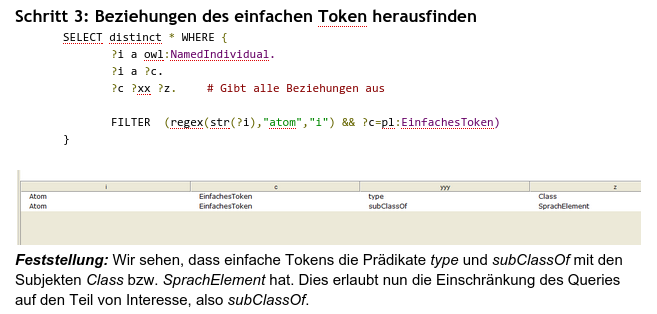
\includegraphics{bilder/sparql_beispiel.png}}}
\caption{Beispiel einer Abfrage der Ontologie mittels SPARQL.\label{fig:sparql_beispiel}\protect\footnotemark}
\end{figure}
\footnotetext{Eigene Darstellung mittels Stanford Protégé und Google Docs.}

Bei den genannten Unvollständigkeiten handelte es sich nicht um Fehler: Die Modellierung drohte ins Uferlose zu entgleiten, da der Detaillierungsgrad der Modellierung nicht abgegrenzt war. Damit zeigte sich: Eine zu feine Granularität kann die Modellierung ins Uferlose führen.\\
Das Ziel der Arbeit war jedoch die Schaffung eines einfachen Systemes und dadurch Erfahrungen mit semantischen Datenbanken und Expertensystemen zu sammeln.

Herr Prof.\ Dr.\ Eckerle empfahl bei der Problembesprechung Inhalte des Buches \textit{Künstliche Intelligenz} von \textit{U. Lämmel} und \textit{J. Cleeve}~\cite{laemmel} als einschränkende Richtlinie zur Modellierung zu verwenden.\\
Das bedeutet Beschränkung der Autoren ausschliesslich auf die Programmiersprache Prolog und deren Kernkonzepte.

Damit konnte eine wesentlich bessere Modellierung mit Klassen, Relationen und Individuen\\
der Ontologie von Prolog erzielt werden.

\begin{figure}[H]
\centering \rotatebox{0}{\scalebox{0.15}[0.15]{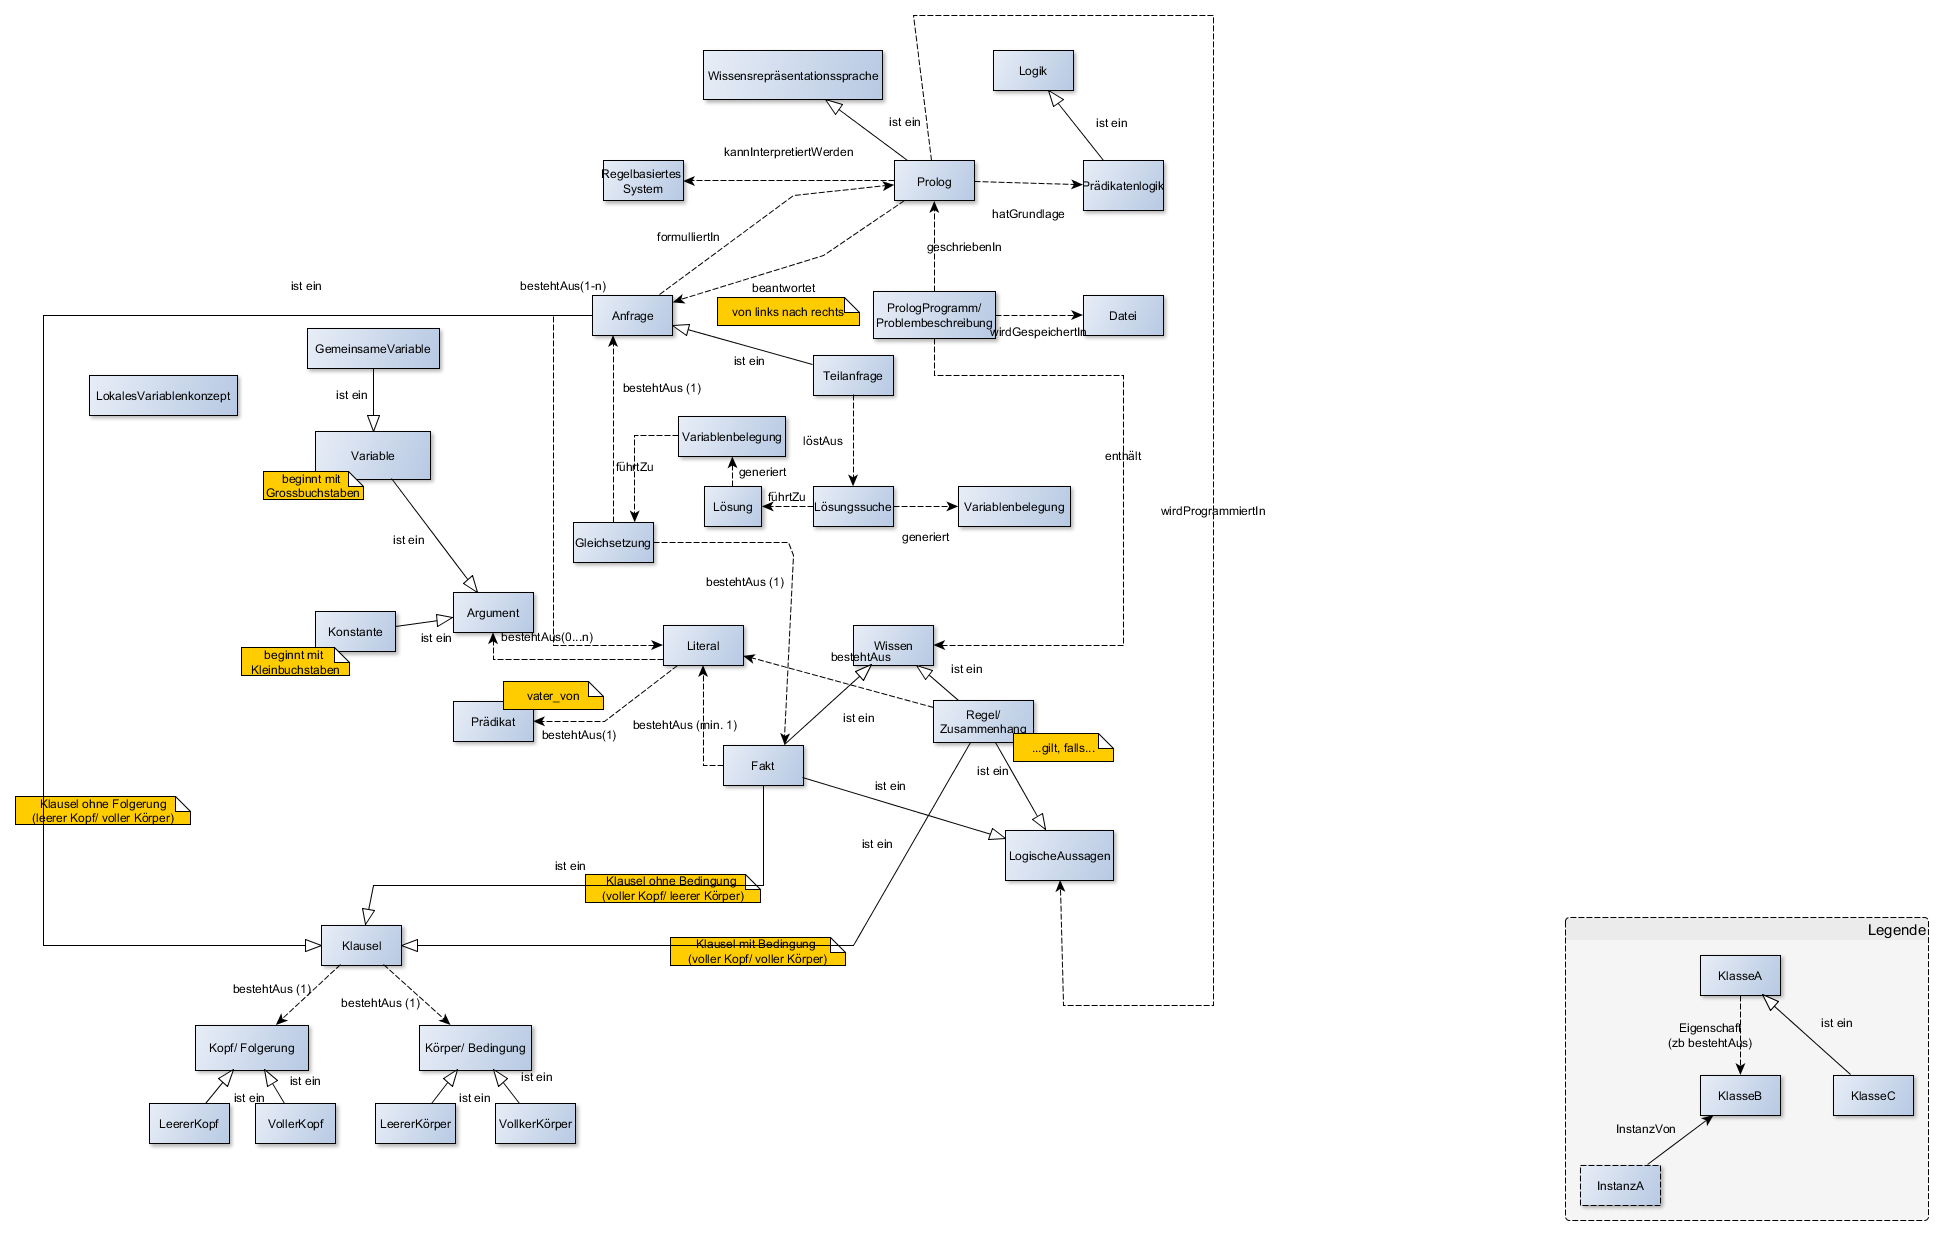
\includegraphics{bilder/prolog_baum.png}}}
\caption{Darstellung der Ontologie von Prolog, mit Klassen und Relationen (Individuen wurden der Übersicht halber bewusst weggelassen).\label{fig:prolog_baum}\protect\footnotemark}
\end{figure}
\footnotetext{Eigene Darstellung mittels yEd.}

Die verbesserte Modellierung bedeutete jedoch keinen Mehrwert in Form von Inferenz. In mehreren Gesprächen bemängelte Herr Prof.\ Dr.\ Eckerle das Fehlen von Regeln in der Ontologie. Um von der objektorientierten Denkweise loszukommen und die Anwendung besser zu verstehen, wurde versucht eine Modellierung der Ontologie direkt in Prolog vorzunehmen. Durch die Struktur von Prolog war die Definition und Anwendung von Regeln einfacher zu verstehen. In Prolog zeigte sich rasch, dass eine Abfrage nach Fakten (ohne Regeln) keinen Mehrwert bringt.

Nach mehreren erfolglosen Versuchen, wurden keine Regeln für die Ontologie gefunden. Daraufhin versuchten die Autoren am Beispiel eines Familienstammbaumes eine neue Ontologie mit geeigneten Regeln aufzubauen. In diesem ``klassischen'' Beispiel~\cite[S. 152]{laemmel} wurde der Mehrwert der Wissensmodellierung mittels Ontologien sogleich ersichtlich.

\begin{figure}[H]
\centering \rotatebox{0}{\scalebox{0.15}[0.15]{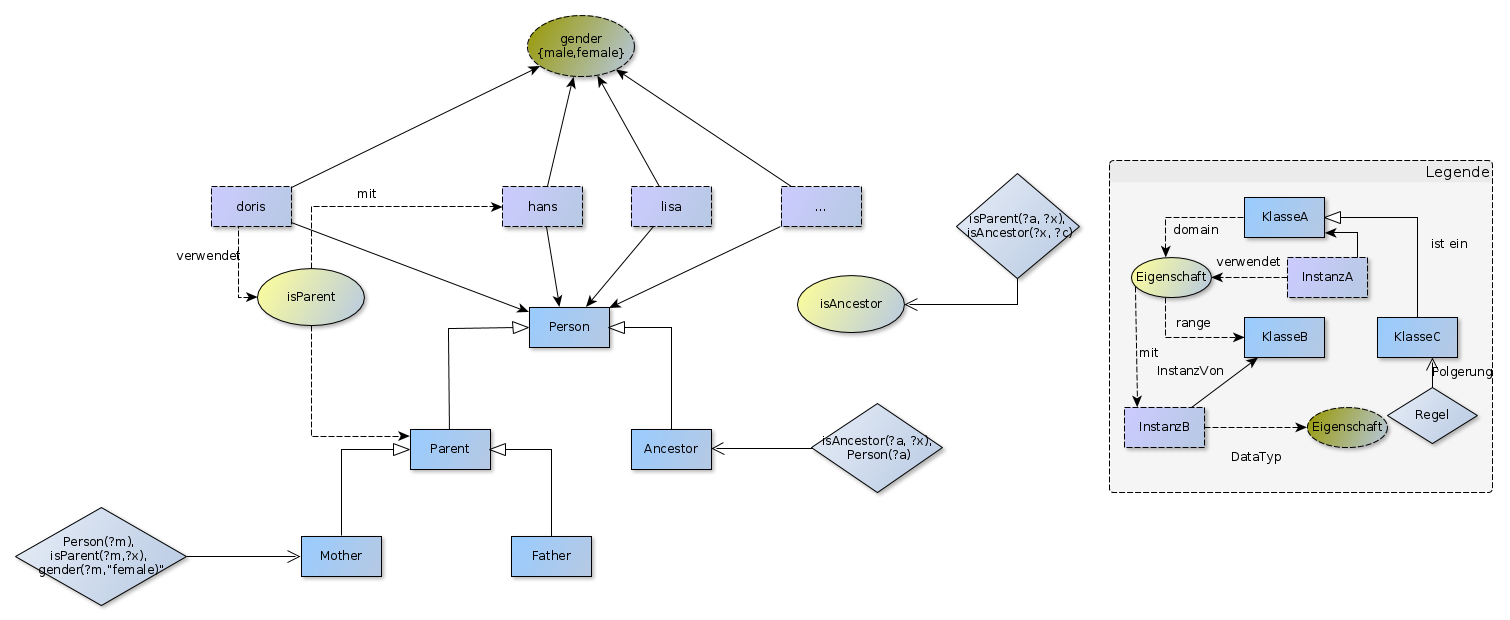
\includegraphics{bilder/familien_netz.png}}}
\caption{Ontologie eines Familienstammbaumes, mit Klassen, Individuen, Relationen und Regeln.\label{fig:familien_netz}\protect\footnotemark}
\end{figure}
\footnotetext{Eigene Darstellung mittels yEd.}

Trotz dieser Erfahrung gelang es nicht, Regeln für die eigentliche Ontologie zu finden. Die Abbildung von Prolog in einer Ontologie ist zwar möglich, jedoch nur in lexikalischer Form. Dies macht den Mehrwert der Wissensmodellierung mittels Ontologien zu Nichte.

Prolog verwendet Unifikation auf Anfragen und setzt dabei Regeln mit Fakten gleich. Bei der Unifikation wird das Konzept Substitution benützt, welches Variablen durch Variablen und/oder Atome substituiert. Die Abbildung der genannten Konzepte in der Modellierung erfolgte hauptsächlich in Form von Fakten (Klassen und Individuen). Zusätzlich konnten einige wenige (komplexe) Regeln gefunden werden.Diese Regeln führen jedoch nicht zu einem Mehrwert.

Das mit diesen Regeln abgebildete Wissen kann auf eine einfachere und intuitivere Weise mittels Fakten abgebildet werden.

Aufgrund obiger Analyse kamen die Autoren zum Schluss, dass sich die gewählte Wissensdomäne (Prolog) nicht für eine Ontologie eignet. Der Mehrwert der Wissensmodellierung mittels einer Ontologie entsteht in diesem Falle nicht.

Für die Wissensmodellierung bzw. Expertensysteme eignen sich besser Wissensdomänen, die aufgrund der Ontologie Inferenz und damit Schlussfolgerungen zulassen. Die ursprünglich gewählte Wissensdomäne befindet sich auf einer zu hohen Abstraktionsebene. Daher ist dort der konkrete Nutzen, in Form von Inferenz, nicht gegeben.

Expertensystem finden entsprechend ihrem Namen dort Anwendung, wo ein Fachexperte erforderlich ist. Durch sein Fachwissen kann der Fachexperte Schlüsse ziehen und damit zusätzliches Wissen beitragen.

Aufgrund der oben ausgeführten Erfahrungen versuchten die Autoren eine neue, geeignete Wissensdomäne zu finden. So wurden zum Beispiel die Planung von Hochzeiten und medizinische sowie pharmazeutische Themengebiete in Betracht gezogen, mangels (Fach-) Wissen aber wieder fallen gelassen.

Als definitive Wissensdomäne wählten die Autoren die Planung von Reisen. Diese Wissensdomäne weist eher in Richtung Expertensysteme. Für Expertensysteme scheinen semantische Netze am geeignetsten zu sein.

\begin{figure}[H]
\centering \rotatebox{0}{\scalebox{0.2}[0.2]{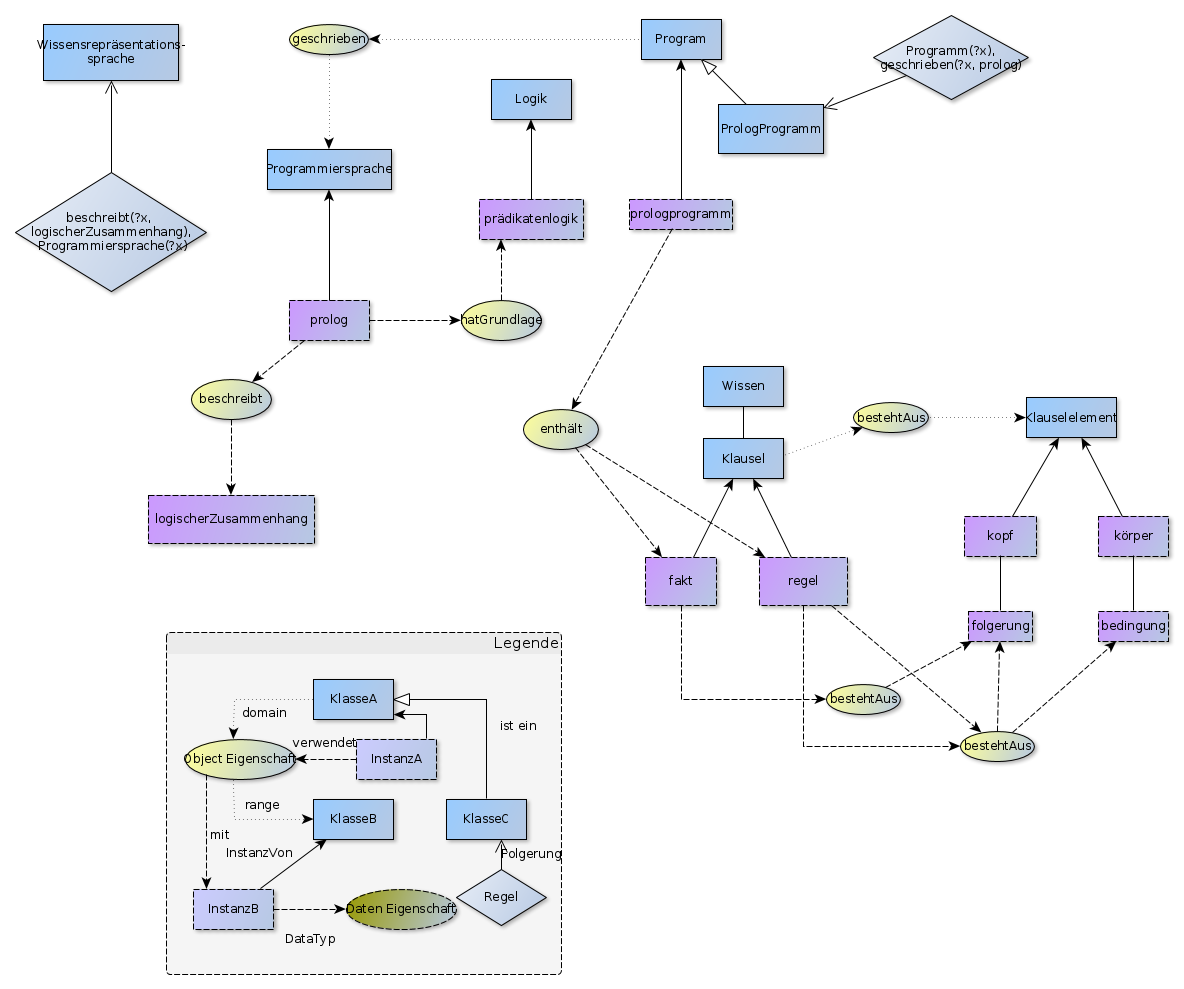
\includegraphics{bilder/prolog_netz.png}}}
\caption{Darstellung eines semantischen Netzes zur Abbildung von Prolog, mit Klassen, Individuen, Relationen und Regeln.\label{fig:prolog_netz}\protect\footnotemark}
\end{figure}
\footnotetext{Eigene Darstellung mittels yEd.}

\subsubsection{Modellierung der tatsächlichen Ontologie}
\label{sub:modellierung_der_ontologie_tatsaechliche}
Das heisst, die Modellierung musste neu aufgebaut werden, dabei konnten aber Erkenntnissen und Erfahrungen aus den Vorversuchen verwendet werden.

Die Autoren entschieden sich zunächst Beispiele zu definieren und erst danach die Modellierung der Ontologie vorzunehmen. Auf den Beispielen basierend wurde die Ontologie erzeugt und stetig erweitert. 

Zur Veranschaulichung ein konkretes Beispiel:

\begin{lstlisting}[caption={Konkretes Beispiel einer Reiseplanung.},captionpos=b]
    Familie Muster plant einen eintägigen Ausflug.
    Die Kinder sind in einem Alter in welchem 
    sie immer beschäftigt werden müssen.
\end{lstlisting}

Die Herleitung des Beispieles findet sich im nachfolgenden Abschnitt. Die zu Grunde liegenden Überlegungen sind im Tutorial aufgeführt.

\newpage

Die Umsetzung des Beispieles führte zu einer sehr einfachen Ontologie, welche in diesem semantischen Netz abgebildet ist:
\begin{figure}[H]
    \centering \rotatebox{0}{\scalebox{0.5}[0.5]{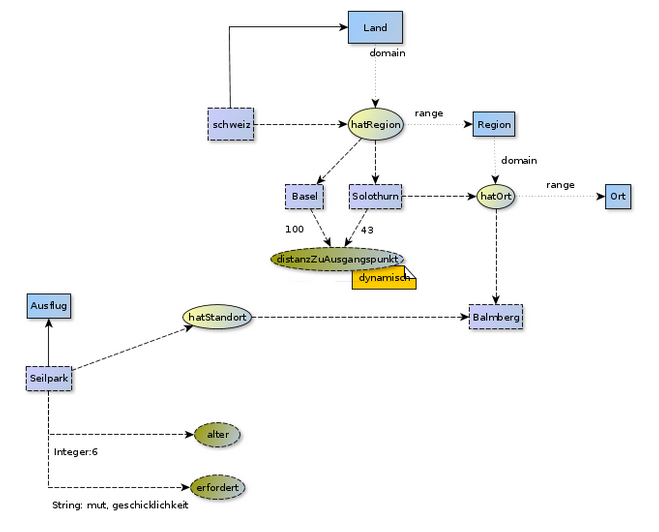
\includegraphics{bilder/famMuster.png}}}
    \caption{Semantisches Netz für den Tagesausflug von Familie Muster.\label{fig:famMuster}\protect\footnotemark}
\end{figure}
\footnotetext{Eigene Darstellung mittels yEd.}

Die Verwendung von Regeln führte in der neu gewählten Wissensdomäne zu einem Mehrwert:
\begin{figure}[H]
    \centering \rotatebox{0}{\scalebox{0.5}[0.5]{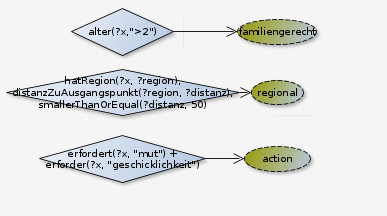
\includegraphics{bilder/famMusterRegeln.png}}}
    \caption{Regeln zu dem semantischen Netz für den Tagesausflug von Familie Muster.\label{fig:famMusterRegeln}\protect\footnotemark}
\end{figure}
\footnotetext{Eigene Darstellung mittels yEd.}

Aus der Modellierung konnten die folgenden Kriterien für die Abfrage abgeleitet werden:

\begin{itemize}
		\item familiengerecht
		\item action
		\item regional
\end{itemize}

Diese sind zugleich die Schlüsse aus den Regeln (Regelkopf). Mittels einer SPARQL-Abfrage wird der Familie Muster schliesslich der Seilpark in Balmberg vorgeschlagen.

\begin{lstlisting}[caption={SPARQL-Abfrage um familiengerechte, regionale und actionreiche Ausflüge zu finden.},captionpos=b,language=SQL]
    SELECT
        *
    WHERE {
        ?object :familiengerecht true;
            :regional true;
            :action true.
        }
\end{lstlisting}


\begin{figure}[H]
\centering \rotatebox{0}{\scalebox{0.5}[0.5]{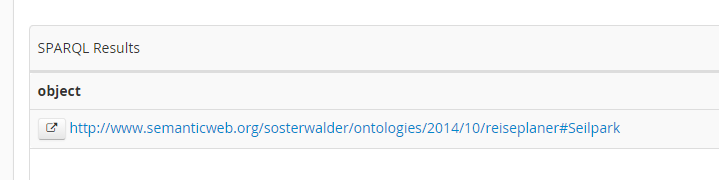
\includegraphics{bilder/famMusterOutput.png}}}
\caption{Ergebnis der Suche von Familie Muster.\label{fig:famMusterOutput}\protect\footnotemark}
\end{figure}
\footnotetext{Eigene Darstellung mittels yEd.}

Damit wird im ausgewählten, bewusst sehr einfach gehaltenen Beispiel, die Herangehensweise der Autoren sichtbar. Bei weiteren, hier nicht aufgeführten Beispielen wurde die Ontologie erweitert.

Zum Beispiel durch Einführung einer Zeiteinheit oder durch eine feinere Rasterung der Eigenschaft familiengerecht. Diese wurde in Untereinheiten aufgeteilt, welche der Altersklasse der Kinder (Kleinkind, Kind oder Teenager) entsprechen.\\
Die gesamte Ontologie wird im~\autoref{sec:loesung_modellierung} genauer erläutert.

\subsection{Tutorialdokument}
\label{subsec:dokumentation_wissensmodellierung}
Gleichzeitig mit der Modellierung der Ontologie entstand ein Tutorial. Das Tutorial zeigt, wie ein Knowledge-Engineer vorgeht um eine Problemdomäne systematisch zu modellieren und formalisieren. Das Tutorial findet sich im Anhang unter~\ref{chap:tutorial}. Da dieses  Tutorial im Gegensatz zu herkömmlichen Tutorials einen grossen Theorieanteil enthält, wurde es nach drei Aspekte aufgeteilt, als da sind:
\begin{itemize}
    \item Theoretisches Hintergrundwissen zur Wissensmodellierung:

        Es wird zum Beispiel erläutert was Expertensysteme sind, wie sie grafisch dargestellt werden können und welche Schreibweisen respektive Sprachen verwendet werden um eine Ontologie abzubilden und darauf Abfragen zu stellen.

    \item Praktische Hinweise zu den jeweiligen Thematiken

        werden im Dokument durch das Symbol Eule gekennzeichnet. Im jeweils danebenstehenden Abschnitt sind praktische Hinweise zur aktuellen Thematik aufgeführt.

    \item Beispiele, wie ein Thema in der Praxis umgesetzt werden kann

        werden im Tutorial durch das Symbol Elefant gekennzeichnet. Sie verkörpern ein Tutorial im klassischen Sinne. Durch Befolgung der aufgeführten Beispiele ist es einem Leser möglich ein simples Beispiel eines Expertensystemes aufzubauen.
\end{itemize}

\subsection{Dokumentation}
\label{subsec:abschliessende_dokumentation}
Die vorliegende Arbeit entspricht der zusammenfassenden Dokumentation. Sie wurde während der gesamten Bachelor-Thesis stetig erweitert. Es diente zur Reflexion von fertiggestellten Teilen.
